\documentclass{article}
\usepackage{physics}
\usepackage{graphicx}
\usepackage{caption}
\usepackage{amsmath}
\usepackage{bm}
\usepackage{framed}
\usepackage{authblk}
\usepackage{empheq}
\usepackage{amsfonts}
\usepackage{esint}
\usepackage[makeroom]{cancel}
\usepackage{dsfont}
\usepackage{centernot}
\usepackage{mathtools}
\usepackage{subcaption}
\usepackage{bigints}
\usepackage{amsthm}
\theoremstyle{definition}
\newtheorem{lemma}{Lemma}
\newtheorem{defn}{Definition}[section]
\newtheorem{prop}{Proposition}[section]
\newtheorem{rmk}{Remark}[section]
\newtheorem{thm}{Theorem}[section]
\newtheorem{exmp}{Example}[section]
\newtheorem{prob}{Problem}[section]
\newtheorem{sln}{Solution}[section]
\newtheorem*{prob*}{Problem}
\newtheorem{exer}{Exercise}[section]
\newtheorem*{exer*}{Exercise}
\newtheorem*{sln*}{Solution}
\usepackage{empheq}
\usepackage{tensor}
\usepackage{xcolor}
%\definecolor{colby}{rgb}{0.0, 0.0, 0.5}
\definecolor{MIT}{RGB}{163, 31, 52}
\usepackage[pdftex]{hyperref}
%\hypersetup{colorlinks,urlcolor=colby}
\hypersetup{colorlinks,linkcolor={MIT},citecolor={MIT},urlcolor={MIT}}  
\usepackage[left=1in,right=1in,top=1in,bottom=1in]{geometry}

\usepackage{newpxtext,newpxmath}
\newcommand*\widefbox[1]{\fbox{\hspace{2em}#1\hspace{2em}}}

\newcommand{\p}{\partial}
\newcommand{\R}{\mathbb{R}}
\newcommand{\C}{\mathbb{C}}
\newcommand{\lag}{\mathcal{L}}
\newcommand{\nn}{\nonumber}
\newcommand{\ham}{\mathcal{H}}
\newcommand{\M}{\mathcal{M}}
\newcommand{\I}{\mathcal{I}}
\newcommand{\K}{\mathcal{K}}
\newcommand{\F}{\mathcal{F}}
\newcommand{\w}{\omega}
\newcommand{\lam}{\lambda}
\newcommand{\al}{\alpha}
\newcommand{\be}{\beta}
\newcommand{\x}{\xi}

\newcommand{\G}{\mathcal{G}}

\newcommand{\f}[2]{\frac{#1}{#2}}

\newcommand{\ift}{\infty}

\newcommand{\lp}{\left(}
\newcommand{\rp}{\right)}

\newcommand{\lb}{\left[}
\newcommand{\rb}{\right]}

\newcommand{\lc}{\left\{}
\newcommand{\rc}{\right\}}


\newcommand{\V}{\mathbf{V}}
\newcommand{\U}{\mathcal{U}}
\newcommand{\Id}{\mathcal{I}}
\newcommand{\D}{\mathcal{D}}
\newcommand{\Z}{\mathcal{Z}}

%\setcounter{chapter}{-1}


\usepackage{enumitem}



\usepackage{listings}
\captionsetup[lstlisting]{margin=0cm,format=hang,font=small,format=plain,labelfont={bf,up},textfont={it}}
\renewcommand*{\lstlistingname}{Code \textcolor{violet}{\textsl{Mathematica}}}
\definecolor{gris245}{RGB}{245,245,245}
\definecolor{olive}{RGB}{50,140,50}
\definecolor{brun}{RGB}{175,100,80}

%\hypersetup{colorlinks,urlcolor=colby}
\lstset{
	tabsize=4,
	frame=single,
	language=mathematica,
	basicstyle=\scriptsize\ttfamily,
	keywordstyle=\color{black},
	backgroundcolor=\color{gris245},
	commentstyle=\color{gray},
	showstringspaces=false,
	emph={
		r1,
		r2,
		epsilon,epsilon_,
		Newton,Newton_
	},emphstyle={\color{olive}},
	emph={[2]
		L,
		CouleurCourbe,
		PotentielEffectif,
		IdCourbe,
		Courbe
	},emphstyle={[2]\color{blue}},
	emph={[3]r,r_,n,n_},emphstyle={[3]\color{magenta}}
}


\begin{document}
\begin{framed}
\noindent Name: \textbf{Huan Q. Bui}\\
Course: \textbf{8.422 - AMO II}\\
Problem set: \textbf{\#5}\\
Due: Friday, Mar 17, 2022\\
References: 
\end{framed}
	


\noindent \textbf{1. Better Phase Measurement with Squeezed Vacuum.}\\

\noindent One application of squeezed light is to measure phase shifts with better precision than can be
achieved with the same number of photons in a coherent state.  In this problem, we employ a
Mach-Zehnder interferometer with coherent and squeezed input states. This interferometer uses two 50/50 beamsplitters and has a phase shift in one path of $\phi$ and has output ports of $b_\text{out}$ and $a_\text{out}$. 

\begin{figure*}[!htb]
\centering
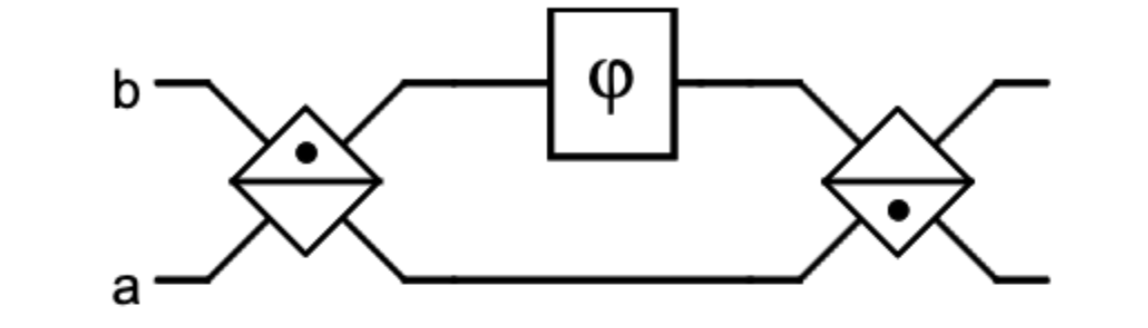
\includegraphics[width=0.4\textwidth]{figures/BS.png}
\end{figure*}



\begin{enumerate}[label=(\alph*)]

\item Suppose the input on port $a$ is a coherent state $\ket{\al}$ and the input on port $b$ is the vacuum state $\ket{0}$. Here we calculate the output signal $\langle M \rangle = \langle b_\text{out}^\dagger b_\text{out} - a_\text{out} ^\dagger a_\text{out} \rangle$, its variance $\langle  \Delta M^2 \rangle = \langle \Delta (b_\text{output}^\dagger b_\text{output} - a_\text{output}^\dagger a_\text{output})^2$, and the signal-to-noise ratio $\langle M \rangle / \sqrt{\langle \Delta M^2 \rangle}$.\\

Let's first compute the output ports in terms of the input ports. After the first beamsplitter, we have 
\begin{align*}
b_1 = BbB^\dagger  = \f{b-a}{\sqrt{2}} \quad\quad \text{and} \quad\quad a_1 = BaB^\dagger = \f{b+a}{\sqrt{2}}.
\end{align*}
Remembering that the beamsplitter with the dot facing up is $B$, we calculate the output after it:
\begin{align*}
B\ket{\al}_a \ket{0}_b = e^{-\abs{\al}^2/2} B e^{\al a^\dagger } B^\dagger \ket{0}_a \ket{0}_b = 
e^{-\abs{\al}^2/2}\exp\lp \al \f{a^\dagger + b^\dagger }{\sqrt{2}} \rp \ket{0}\ket{0} = 
\ket{\f{\al}{\sqrt{2}} }_{a_1} \ket{ \f{\al}{\sqrt{2}}}_{b_1}.
\end{align*}
After the phase shift in the $b$ mode we have
\begin{align*}
\ket{\f{\al}{\sqrt{2}} }_{a_1} \ket{ \f{\al}{\sqrt{2}}}_{b_1} \to \
 \ket{\f{\al}{\sqrt{2}} }_{a_1} \ket{ \f{\al e^{i\varphi}}{\sqrt{2}}}_{b_1}.
\end{align*}
Finally, we apply $B^\dagger$ to this state: 
\begin{align*}
B^\dagger  \ket{\f{\al}{\sqrt{2}} }_{a_1} \ket{ \f{\al e^{i\varphi}}{\sqrt{2}}}_{b_1} 
&= e^{-\abs{\al}^2/2} B^\dagger e^{\al a^\dagger  /\sqrt{2}} e^{\al e^{i\varphi} b^\dagger  /\sqrt{2}  } BB^\dagger \ket{0} \ket{0} \\
&= e^{-\abs{\al}^2/2} \exp\lp \f{\al}{2}(  a^\dagger - b^\dagger)  + \f{\al e^{i\varphi}}{2}(a^\dagger + b^\dagger ) \rp  \ket{0} \ket{0}\\
&= e^{-\abs{\al}^2/2} \exp\lp a^\dagger \f{\al(1 + e^{i\varphi})}{2} + b^\dagger \f{\al(-1 + e^{i\varphi})}{2} \rp \ket{0} \ket{0}\\
&= \ket{\f{\al(1+e^{i\varphi})}{2}}_{a_\text{out}} \ket{\f{\al(-1+e^{i\varphi})}{2}}_{b_\text{out}}.
\end{align*}
With this we can compute the signal:
\begin{align*}
\langle M \rangle = \langle b_\text{out}^\dagger b_\text{out} - a_\text{out}^\dagger a_\text{out} \rangle 
= \langle b_\text{out}^\dagger b_\text{out} \rangle - \langle a_\text{out}^\dagger a_\text{out} \rangle 
= \f{\abs{\al}^2}{4}\abs{-1+e^{i\varphi}}^2  - \f{\abs{\al}^2}{4} \abs{1+e^{i\varphi}}^2 
= - \abs{\al}^2 \cos\varphi 
\end{align*}
Next we compute the variance in the signal:
\begin{align*}
\langle \Delta M^2 \rangle 
&= \langle M^2\rangle - \langle M \rangle^2\\ 
&= \langle (b_\text{out}^\dagger b_\text{out} - a_\text{out}^\dagger a_\text{out})^2 \rangle - \abs{\al}^4\cos^2\varphi \\ 
&= \langle  b_\text{out}^\dagger b_\text{out} b_\text{out}^\dagger b_\text{out} + 
a_\text{out}^\dagger a_\text{out}a_\text{out}^\dagger a_\text{out}  
- 2 b_\text{out}^\dagger b_\text{out}a_\text{out}^\dagger a_\text{out} \rangle - \abs{\al}^4 \cos^2\varphi\\ 
&= \langle n^2_{b,\text{out}} \rangle + \langle n^2_{a,\text{out}} \rangle 
-2 \langle n_{b,\text{out}} \rangle  \langle n_{a,\text{out}} \rangle - \abs{\al}^4 \cos^2 \varphi \\ 
&= \abs{\f{\al(-1 + e^{i\varphi})}{2}}^4 + \abs{\f{\al(-1 + e^{i\varphi})}{2}}^2 
+ \abs{\f{\al(1+ e^{i\varphi})}{2}}^4 + \abs{\f{\al(1+ e^{i\varphi})}{2}}^2 \\
&\quad - 2 \abs{\f{\al(-1 + e^{i\varphi})}{2}}^2 \abs{ \f{\al(1 + e^{i\varphi})}{2}}^2 
- \abs{\al}^4\cos^2\varphi\\
&= \f{\abs{\al}^4}{16}( 16 \cos^2\varphi  ) - \abs{\al}^4 \cos^2\varphi
+ \f{4\abs{\al}^2}{4}\\
&= \abs{\al}^2.
\end{align*}
With these, the sign-to-noise ratio in the signal is 
\begin{align*}
\text{SNR} = \abs{ \f{\langle M\rangle}{\sqrt{\langle \Delta M^2 \rangle}} }= \f{\abs{\al}^2 \abs{ \cos\varphi}}{\abs{\al}} = \abs{\al \cos\varphi}.
\end{align*}



\item The minimal detectable phase is the phase $\phi_\text{min}$ for which $\text{SNR} = 1$. Assuming we have a strong coherent state then $\cos \varphi$ is small. This means we want to expand $\cos \varphi$ near $\pi/2$.
\begin{align*}
1 = \abs{\al} \cos\varphi_\text{min} \approx  \pm \abs{\al} \lp \varphi_\text{min} - \f{\pi}{2}  \rp \implies \varphi_\text{min} \approx \pm \f{1}{\abs{\al}} + \f{\pi}{2}.
\end{align*}

\item Now we repeat the calculation but with the squeezed vacuum $S(r) \ket{0}$ entering port $b$ instead. In view of the last problem set where we decomposed the squeezing operator into 
\begin{align*}
S(r) = e^{\f{r}{2}({ b^\dagger}^2 - b^2) } = e^{\f{u}{2} {b^\dagger}^2} e^{ t (b^\dagger b + 1/2)} e^{\f{v}{2} a^2}
\end{align*}
with $u = - v  = \tanh r$ and $t  =-\ln \cosh r $, we find that
\begin{align*}
B\ket{\al}_a S(r) \ket{0}_b 
&= \f{e^{-\abs{\al}^2/2}}{\sqrt{\cosh r}} B e^{\al a^\dagger }  e^{\f{\tanh r}{2} {b^\dagger}^2} \ket{0}_a \ket{0}_b.
\end{align*}
Note here that the terms with $t,v$ act as identities on the vacuum state, so only the $u$ term remains. Under the beamsplitter transformation $B\cdot B^\dagger$, we have
\begin{align*}
\f{e^{-\abs{\al}^2/2}}{\sqrt{\cosh r}}  B\ket{\al}_a S(r) \ket{0}_b 
\to 
\f{e^{-\abs{\al}^2/2}}{\sqrt{\cosh r}}  e^{\f{\al}{\sqrt{2} }(a^\dagger + b^\dagger)} e^{\f{\tanh r }{4} (b^\dagger - a^\dagger)^2   } \ket{00} 
\end{align*}
We notice that the 



\item 

\end{enumerate}



\noindent \textbf{2. Hanbury-Brown and Twiss Experiment with Atoms.}  \\

\noindent This problem illustrates the coherence and collimation requirements for performing a Hanbury
Brown and Twiss (HBT) experiment with atoms.  If a free particle starts at point $A$ at time $t=0$ with amplitude $\psi_A$ then the amplitude at another point $1$ and time $t = \tau$ is proportional to $\psi_A e^{i( \vec{k}\cdot \vec{r}_{A1}  -\omega \tau)}$. 

\begin{enumerate}[label=(\alph*)]

\item \textbf{Correlation function.} Assume we have a particle at $A$ with amplitude $\psi_A$ and a particle at $B$ with amplitude $\psi_B$. Then the joint probability $P$ of finding one particle at $A$ and one particle at $B$ is 
\begin{align*}
P = \abs{\psi_A e^{i\phi_{A1}}   \psi_B  e^{i\phi_{B2}} \pm \psi_A e^{i\phi_{A2}} \psi_B e^{i\phi_{B1}} }^2
\end{align*}
and is proportional to the second-order coherence function $g^{(2)}(1,2)$. The $\pm$ is for bosons/fermions. Here, $\phi_{A1} = \vec{k}_A \cdot r_{A1}  -\omega \tau$, etc. Here we want to calculate $P$ as a function of $\vec{r}_{21}$, the vector from point $2$ to point $1$ on the detector. To do this, we simply put:
\begin{align*}
\vec{r}_{B1} =  \vec{r}_{B2} + \vec{r}_{21} \quad\quad \text{and} \quad\quad \vec{r}_{A2} = \vec{r}_{A1} - \vec{r}_{21}. 
\end{align*}
From these, we find 
\begin{align*}
P 
&= \abs{  \underbrace{ \psi_A \psi_B e^{-2i\omega \tau} e^{i\vec{k}_A \cdot \vec{r}_{A1}}  e^{i\vec{k}_B \cdot \vec{r}_{B2}} }_{C}
\pm
\underbrace{\psi_A \psi_B e^{-2i\omega\tau} e^{i\vec{k}_A \cdot \vec{r}_{A1} } e^{i\vec{k}_B\cdot \vec{r}_{B2}}}_{C}
e^{-i\vec{k}_A \cdot \vec{r}_{21}} e^{i\vec{k}_B \cdot \vec{r}_{21} } 
}^2 \\
&= \abs{C(1 \pm e^{-i\vec{k}_A \cdot \vec{r}_{21}} e^{i\vec{k}_B \cdot \vec{r}_{21} }  )}^2 \\ 
&= \abs{\psi_A \psi_B}^2 \abs{1 \pm e^{i(\vec{k}_B - \vec{k}_A ) \cdot \vec{r}_{21}   }}^2.
\end{align*}

\item \textbf{Transverse collimation.} Assume that we are given a source with transverse dimension $W$ and detector with transverse dimension $w$ where $\vec{r}_{21} \leq w$. The distance between the source and the detector $d$ is much greater than all other distances. The transverse component of the phase factor from part (a) can be written as $\phi_t = (\vec{k}_A - \vec{k}_B)_t \cdot (\vec{r}_{21})_t$. Assume that the signal at
the detector is mainly due to atoms with wavevectors distributed around $\vec{k}_0$. \\

\noindent  As seen from the detector, the angular size of the source is given by $W/d$. In order to see second-order correlation effects, the de Broglie wavelength of the particles, after taking into account the angular size of the target due to being at a distance $d$ away from the detector, must be much larger than the detector size.  As a result, we must have that 
\begin{align*}
w \ll \f{\lambda_{dB}}{W/d} \implies Ww \ll d \lambda_{dB},
\end{align*}
as desired. This is related to the transverse collimation requirement. \\


\noindent Now we consider a $^6$Li MOT at 500 \textmu K. The de Broglie wavelength is 
\begin{align*}
\lambda_{dB} = \f{h}{p} = \f{h}{\sqrt{2\pi m_{^6\text{Li}} k_BT}} \approx 3.18 \times 10^{-8} \text{ m} = 31.8 \text{ nm}. 
\end{align*}
Assuming the MOT and detector have equal size, i.e., $W \approx w$, then an upper bound on the magnitude of $W\approx w$ is simply 
\begin{align*}
\sqrt{d\lambda_{dB}} \approx 0.000056 \text{ m} = 56 \text{ \textmu m}
\end{align*}
where we have used $d=10$ cm. 




\item \textbf{Longitudinal collimation}

\item \textbf{Phase-space volume enhancement}

\end{enumerate}





\end{document}








